\documentclass[../../main.tex]{subfiles}

\begin{document}

% \begin{abstract}
% Design of high performance, high abstraction libraries in \cpp often take
% advantages of techniques like template metaprogramming or expression templates
% to design \dsels{.} However, such techniques are limited by the natural syntax
% of \cpp. In this paper, we explore the benefits of using \cpp23 compile time
% computation features to provide compile time string based \dsels that can then
% use arbitrary syntax.
% \end{abstract}

\chapter{Arbitrary syntax languages embedding in C++23}

\cpp is often touted as a \textit{Zero-Cost Abstraction} langage due to some of
its design philosophy and its ability to compile abstraction to a very efficient
binary code. Some more radical techniques can be used to force the compiler to
interpret \cpp code as a \dsel. Template metaprogramming is such a technique
and it spawned a large corpus of related idioms from compile time function
evaluation to lazy evaluation via \textit{Expression Templates}.\\

In the field of High Performance Computing, \cpp users are often driven to use
libraries built on top of those idioms like Eigen\cite{eigen} or
Blaze\cite{blazelib,iglberger2012_2}. They all suffer from a major limitation:
by being tied to the natural \cpp syntax, they can't express nor embed arbitrary
languages.\\

In this paper, we try to demonstrate that the new features of \cpp23 related to
compile time programming are able to help developers designing \dsels with
arbitrary syntax by leveraging \constexpr computations, compile time dynamic
objects and lazy evaluation through lambda functions. After contextualizing our
contribution in the general \dsels domain, this paper will explain the core
new techniques enabled by \cpp23 and how we can apply to build two different
\dsels with their own non-\cpp syntax. We'll also explore the performances of
said \dsels in term of compile time to assess their usability in realistic code.

\section{State of the art}

By definition, a Domain-Specific Language (\dsl) is a computer language
specialized to a particular application domain, contrary to a general-purpose
language, which is broadly applicable across domains, and lacks specialized
features for a particular domain. Domain Specific Embedded Languages (\dsels)
are a subclass of \dsl that rely on an existing general-purpose language to host
it. \dsels then reuse the host language syntax and tool ecosystem to be compiled
or interpreted.\\

In \cpp, the compile time process of generating new code is \textbf{Template
Metaprogramming} to ensure performances and correctness.

% TODO: Merge with state of the art chapter

% \subsection{Template Metaprogramming}
%
% \cpp template metaprogramming \cite{abrahams:2004} is a technique based on the
% use of the template type system of \cpp to perform arbitrary computation at
% compile time. This property of \cpp templates is due to the fact they
% define a Turing-complete sub-language manipulating types and integral constants
% at compile time \cite{unruh:1994}. Due to the fact that template code generation
% is performed at compile time, uses constants and supports pattern-matching and
% recursion thanks to template partial specialization, it can also be looked
% at as a pure functional language \cite{haeri:2012}.\\
%
% Templates are an interesting technique for generative programming. As they
% are Turing-complete, one can design a set of template metaprograms acting as a
% \dsl compiler run at compile time and generating temporary \cpp code fragment as
% an output. The resulting temporary source code is then merged with the rest of
% the source code and finally processed by the classic compilation process.
% Through this technique, compile time constants, data structures and complete
% functions can be manipulated. The execution of metaprograms by the compiler
% enables the library to implement domain-specific optimizations that lead to a
% complete domain oriented code generation. Such a technique can be hosted by
% several languages featuring metaprogramming features (incidental or by design)
% like D \cite{template:dlang}, Haskell \cite{sheard:2002} and
% OCaml \cite{serot:2008}.

\subsection{C++ Domain Specific Embedded Languages}

\dsels in \cpp use template metaprogramming via the \textit{Expression
Template} idiom.
\textbf{Expression Templates} \cite{veldhuizen:1995,vandevoorde:2002} is a
technique implementing a
form of \textbf{delayed evaluation} in \cpp \cite{spinellis:2001}. Expression
Templates are built around the \textit{recursive type composition}
idiom \cite{jarvi:1998} that allows the construction, at compile time, of a type
representing the abstract syntax tree of an arbitrary statement. This is done by
overloading functions and operators on those types so they return a lightweight
object. The object encodes the current operation in the Abstract Syntax Tree
(AST) being built in its type instead of performing any kind of computation. Once
reconstructed, this AST can be transformed into arbitrary code fragments using
Template Metaprograms.\\

As of today, most \cpp EDSLs rely on \textit{Expression Templates} and therefore
are limited to the \cpp syntax. New techniques are becoming more popular through
the use of \constexpr strings to embed arbitray \dsels{.} One major example is
the Compile-Time Regular Expressions library (CTRE)\cite{ctre} that implements
most of the Perl Compatible Regular Expression (PCRE) syntax. However, CTRE
still relies on type-based template metaprogramming to parse regular expressions
and transform them into regular expression evaluators.

% https://martinfowler.com/books/dsl.html

\section{C++23 constexpr programming and constexpr memory allocation}

Since the introduction of the \constexpr specifier with \cpp11, the requirements
for functions to be \constexpr specifiable have constantly been relaxed as new
\cpp standards were adopted. In \cpp20, notable changes made dynamic memory
allocations\cite{constexpr-memory} and virtual \constexpr function
calls\cite{virtual-constexpr} allowed in \constexpr function
bodies. These two additions make dynamic memory and heritage-based polymorphism
possible in \constexpr functions. Therefore more regular \cpp code can be
executed at compile time, including parsers for arbitrary languages.

\subsection{The constexpr qualifier}

The \constexpr qualifier can be applied on variables and functions. It means
that they can be used in the context of constant evaluation, \ie they can be
used to generate other compile time constants such as \constexpr variables
or non-type template parameters (NTTP).

\paragraph{Constexpr functions} Functions that are \constexpr qualified can
still be used in other contexts than constant evaluation happening at
compile time. In non-constant evaluation, \constexpr functions can still call
non-\constexpr functions. But in constant evaluation, \constexpr functions can
only call other \constexpr functions.


\paragraph{Constexpr variables} Variables that are \constexpr qualified can be
used in constant expressions. Note that they are different from
non-\constexpr variables used in \constexpr functions.


\paragraph{Constexpr memory allocation} Starting from \cpp20,
\lstinline|std::allocate| and \lstinline|std::deallocate| are
\constexpr functions, allowing memory allocations to happen in constant
evaluation. However,
\constexpr allocated memory is not transient, \ie memory allocated in
constant expressions cannot be stored in \constexpr variables.
The use of any value that holds a pointer to \constexpr allocated memory as a
non-type template parameter is also prohibited (listing \ref{cxexamples}).

\begin{lstlisting}[
  language=C++,
  caption=Illustration of constraints on \constexpr allocated memory,
  label=cxexamples
]
template<auto> constexpr int foo() { return 1; }
constexpr std::vector<int> generate() { return {1,2,3,4,5}; }

constexpr auto a = generate();        // Error
constexpr auto b = generate().size(); // OK
constexpr auto c = foo<generate()>(); // Error
constexpr auto d = foo<&generate>();  // OK
\end{lstlisting}

Notice how the last example works around restrictions of \constexpr allocations
by using a generator function instead of passing a non-empty
\lstinline|std::vector<int>| value directly.


\paragraph{Constexpr virtual functions} This feature allows calls to virtual
functions in constant expressions\cite{virtual-constexpr}. This allows
heritage-based polymorphism in \constexpr programming when used with
\constexpr allocation of polymorphic types.

\subsection{Cest: standard-like containers for constexpr programming}

As of today not all standard containers can be used in constant expressions.
It is the case for \lstinline{std::map}, \lstinline{std::set}, and others,
making some \cpp programs harder to adapt for use in constant evaluations.\\

The Cest\cite{cest} project was started by Paul Keir to tackle this issue
by providing containers that are interchangeable with the ones present
in the C++ standard library, and are usable in constant expressions.

Even though the Poacher project does not depend on Cest anymore,
it has been instrumental to start experimenting with \constexpr programming
at the beginning of my thesis. It took time for standard libraries such as
GNU's stdlibc++ and LLVM's libc++ to implement \constexpr compatibility for
\lstinline{std::vector} (standardized in \cpp20) or \lstinline{std::unique_ptr}
(standardized in \cpp23), and my motivation was to use implement \constexpr
parsers with very limited use of unconventional programming techniques.

For example, some \constexpr programs or libraries use \lstinline{std::array}
as an alternative to \lstinline{std::vector} in \constexpr function bodies
as \lstinline{std::array} was made compatible for use in \constexpr functions
as soon as \cpp17. However, the use of preallocated arrays requires workarounds
such as using additional variables to keep track of element count,
additional computations to estimate a lower bound for preallocation,
or simply using arbitrary "magic" values for preallocations.
Moreover, assigning static arrays of different sizes is not permitted,
adding more unnecessary complexity to \constexpr functions.\\

I contributed to the Cest project by implementing the \constexpr compatible
alternative to \lstinline{std::unique_ptr}, which was essential for the
implementation of the Brainfuck \constexpr parser in \ref{lbl:bf-frontend}.

\section{C++23 experiments for implementing EDSLs of arbitrary syntaxes}

We explore two cases of \constexpr parser implementations for small languages
that return abstract syntax trees using \constexpr allocated memory through
standard containers, and backends that transform the \constexpr function results
into programs through templates using different techniques. The use cases we
consider are:

\begin{itemize}
  \item The Brainfuck as a Turing machine emulation language. Its main interest
        is its large corpus of example programs.
  \item A basic math language supporting infix operators and function calls.
\end{itemize}

The Poacher project was started to experiment ways to leverage \constexpr
programming for the integration of embedded domain specific languages of
arbitrary syntaxes. Considering the current restrictions on \constexpr allocated
memory, going from a static string representation of a program, mathematical formula, or
regular expression to a compiled program using \constexpr programming might not
be trivial.

% https://www.cs.rhul.ac.uk/research/languages/csle/lookahead_backtrack.html
% https://www.boost.org/doc/libs/1_81_0/libs/spirit/doc/html/spirit/references.html
% https://github.com/antlr/antlr4

\section{Brainfuck as a C++ DSEL}

Brainfuck (as known as BF) is a structured imperative language characterized by
8 tokens that allow increasing or decreasing a pointer to single byte values in
a fixed size array, acting on the pointee value by increasing or decreasing it,
single character input/output, and looping as long as the pointee value is
non-zero. Each one of its instructions can be translated directly into
\cpp code (see table \ref{fig:BF}).

\begin{figure}[h]
\begin{tabular}{|l|l|}
\hline
BF token & \cpp equivalent \\ \hline
(Program start) & \lstinline|char array[30000] = {0}; char *ptr = array;| \\
\lstinline|>| & \lstinline|++ptr;| \\
\lstinline|<| & \lstinline|--ptr;| \\
\lstinline|+| & \lstinline|++*ptr;| \\
\lstinline|-| & \lstinline|--*ptr;| \\
\lstinline|.| & \lstinline|std::putchar(*ptr);| \\
\lstinline|,| & \lstinline|*ptr = std::getchar();| \\
\lstinline|[| & \lstinline|while (*ptr) {| \\
\lstinline|]| & \lstinline|}| \\
% Any other token & Nothing \\
\hline
\end{tabular}
\caption{
  BF token to \cpp code conversion table --
  https://en.wikipedia.org/wiki/Brainfuck
}
\label{fig:BF}
\end{figure}

Our objective with this metacompiler is to go from abstract syntax trees built
using \constexpr dynamic structures to runtime code. The first part of this case
study will cover the frontend, \ie the AST structure and the parser, then the
second part will cover the two backends that implement different code generation
strategies.

% http://esoteric.sange.fi/brainfuck/utils/mandelbrot/

\subsection{Frontend design} \label{lbl:bf-frontend}

The first building blocks that must be represented by the BF AST are the
instructions. A trivial kind of representation that can be used in constant
expressions are enum types. Because BF instructions are single character tokens,
we decided to simply call them "tokens" in our syntactic representation.

\lstinputlisting[
  language=C++,
  firstline=12,
  lastline=22,
  caption=\lstinline|token_t| enum type definition,
  label=lst:token_t
]{external/poacher/brainfog/include/brainfog/ast.hpp}

Note that the language has to support loops, and eventually nested loops.
To represent them properly, we will use a polymorphic tree representation.
Since \cpp20 allows virtual functions and dynamic memory, these can be
implemented using inheritance, which is a fairly common way to represent AST
nodes.\\

The next step then is to define 3 kinds of AST nodes: single tokens (\ie single
instructions), instruction blocks, and loops. They all inherit
\lstinline|node_interface_t|, which keeps track of the kind of underlying node
using a value of type \lstinline{ast_node_kind_t}
(listing \ref{lst:node_interface_t}).

\begin{lstlisting}[
  language=C++,
  caption=\lstinline|node_interface_t| definition,
  label=lst:node_interface_t
]
enum ast_node_kind_t { ast_token_v, ast_block_v, ast_while_v };

struct node_interface_t {
private:
  ast_node_kind_t kind_;
protected:
  constexpr node_interface_t(ast_node_kind_t kind) : kind_(kind){};
public:
  constexpr ast_node_kind_t get_kind() const { return kind_; }
  constexpr virtual  node_interface_t() = default;
};
\end{lstlisting}

% \lstinputlisting[
%   language=C++,
%   firstline=61,
%   lastline=73,
%   caption=\lstinline|node_interface_t| definition,
%   label=lst:node_interface_t
% ]{external/poacher/brainfog/include/brainfog/ast.hpp}

Note that all methods are \constexpr, including the constructor and the virtual
destructor. Code blocks and while loops were kept as two separate entities.

% \lstinputlisting[
%   language=C++,
%   caption=\lstinline|ast_node_kind_t| definition,
%   label=lst:ast_node_kind_t
% ]{external/poacher/brainfog/include/brainfog/ast.hpp}

The underlying node types are then defined as follows:

\begin{itemize}
\item \lstinline|ast_token_t|: constains a single token (though they cannot
      contain all tokens as loop begin and end tokens parsed into
      \lstinline|ast_while_t| nodes).
\item \lstinline|ast_block_t|: constains a
      \lstinline|std::vector<cest::unique_ptr<ast_node_kind_t>>|, \ie a vector
      of AST nodes.
\item \lstinline|ast_while_t|: constains an \lstinline|ast_block_t|.
\end{itemize}

These three kinds of nodes are enough to represent programs written in our
rudimentary, yet structured and Turing-complete language. Now we'll take a look
at the \constexpr parser implementation.

\subsection{A constexpr parser for the BF language}

The parser itself is relatively simple and can be used to parse BF programs at
runtime as it is a regular \cpp function. The only particularity it has is its
\constexpr qualification, and thus its reliance on \constexpr functions
exclusively.

\begin{lstlisting}[
  language=c++,
  caption=\lstinline{lex_tokens} function definition,
  label=lst:bf-lex_tokens
]{}
constexpr token_vec_t lex_tokens(std::string const &input) {
  token_vec_t result;
  result.reserve(input.size());
  std::transform(
      input.begin(), input.end(),
      std::back_inserter(result),
      [](char current_character) {
        return to_token(current_character);
      });
  return result;
}
\end{lstlisting}

The first step of BF parsing consists in converting characters
into typed BF tokens. As you can see in listing \ref{lst:bf-lex_tokens}
the transformation is fairly trivial as algorithms from the \cpp standard
library are \constexpr since \cpp20.

\begin{lstlisting}[
  language=c++,
  caption=\lstinline{parse_block} function definition,
  label=lst:bf-parse_block
]{}
constexpr std::tuple<ast_block_t,
                     token_vec_t::const_iterator>
parse_block(token_vec_t::const_iterator parse_begin,
            token_vec_t::const_iterator parse_end) {
  using input_it_t = token_vec_t::const_iterator;

  ast_node_vec_t block_content;

  for (; parse_begin != parse_end; parse_begin++) {
    // While end bracket: return block content
    // and while block end position
    if (*parse_begin == while_end_v) {
      return {std::move(block_content), parse_begin};
    }

    // While begin bracket: recurse,
    // then continue parsing from the end of the block
    else if (*parse_begin == while_begin_v) {
      // Parse while body
      auto [while_block_content, while_block_end] =
          parse_block(parse_begin + 1, parse_end);

      block_content.push_back(
          std::make_unique<ast_while_t>(
            std::move(while_block_content)));

      parse_begin = while_block_end;
    }

    // Any other token that is not a nop instruction:
    // add it to the AST
    else if (*parse_begin != nop_v) {
      block_content.push_back(
          ast_node_ptr_t(
            std::make_unique<ast_token_t>(
              *parse_begin)));
    }
  }

  return {ast_block_t(std::move(block_content)),
          parse_end};
}
\end{lstlisting}

Listing \ref{lst:bf-parse_block} shows the parser's main function.
The function has a main loop that traverses tokens until it finds the end


Thanks to the simplicity of the BF language, it remains very simple
and can be contained in less than 50 lines of code.
Moreover, its the BF metacompiler did not require any template metaprogramming
up to this point. This is a strong argument in favor of using \constexpr
functions for metaprogramming. Template metaprogramming is perceived as a niche
practice and


The output of \lstinline|parse_block| is a
\lstinline|std::tuple<ast_block_t, token_vec_t::const_iterator>|. The first
element of the tuple is the content that was parsed by the function, and the
second element is an iterator pointing after the last parsed element. While
loops are parsed by calling the function recurisvely, and the function returns a
block when it detects a while end token. As you may notice, the parser and AST
implementations were kept as ordinary as possible, as the goal of the
project is to study metaprogramming --and especially code generation-- using
ordinary \cpp constructs instead of template metaprogramming.\\

Now that we have a \constexpr parser, we'll have a look at how to transform its
results into programs.

\subsection{Code generator for the BF language}

Once parsed, the AST has to be transformed into \cpp code. The project currently
has three working backends implementing different strategies. Other
non-working backends served as implementation attempts to better understand the
limitations of \cpp23 for transforming an AST that contains non-transient
allocated memory into \cpp code, but also attempts at using experimental
features proposed to the \cpp standard such as reflection and
splicing\cite{scalable-reflection}.\\

This paper will not detail the failed attempts. We will start with an approach
relying on generators to convert the AST directly into code, another one where
we add a type-based expression template intermediate representation, and another
one that serializes the AST into a representation that is compatible with
non-type template parameters constraints.

\subsubsection{Pass-by-generator backend}

Despite values containing \constexpr allocated memory not being storable in
\constexpr variables, lambda functions that generate them can be stored in
\constexpr variables and used as NTTP. The following example shows how to use
this technique to convert a non-literal \constexpr value into an equivalent
type-based representation, more suitable for code generation.\\

First we define a binary tree data structure that can be used in
\constexpr evaluation called \lstinline|tree_t| and a
\constexpr function called \lstinline|gen_tree| that generates an arbitrary
\lstinline|tree_t| value (listing \ref{lst:tree_t}).

\lstinputlisting[
  language=C++,
  firstline=4,
  lastline=22,
  caption=\lstinline|tree_t| and \lstinline|gen_tree| definitions,
  label=lst:tree_t
]{chapters/poacher/cpp-examples/tree-pass-by-generator.cpp}

As stated earlier, our goal is to generate a program that evaluates the content
of the tree. However, we cannot use the result of \lstinline|gen_tree| directly
as a non-type template parameter. The solution is to pass lambdas that evaluate
its subobjects in a lazy way. In listing \ref{lst:codegen} we demonstrate this
technique by defining a function template that takes a \lstinline|tree_t|
generator function as a template parameter and returns a function that evaluates
the sum of its elements.\\

This technique can be applied to generate expression templates as well.
This is interesting as it makes \constexpr programming interoperable with
existing metaprogramming libraries based on template metaprogramming.

\lstinputlisting[
  language=C++,
  firstline=27,
  lastline=46,
  caption=\lstinline|codegen| definition,
  label=lst:codegen
]{chapters/poacher/cpp-examples/tree-pass-by-generator.cpp}

\subsubsection{Expression template backend}

We first define a type-based tree representation based on an expression template
structure similar to what libraries like Blaze\cite{blazelib} or
Eigen\cite{eigen} already use. To convert the result of \lstinline|gen_tree|
into an expression template, we implement a recursive
function template (listing \ref{lst:to_expression_template}) that takes a
generator function as a non-type template parameter and returns the expression
template equivalent to the generator's result. The equivalence can be tested
at compile time using \lstinline|static_assert| and \lstinline|std::is_same|.

\subsubsection{NTTP backend}

Another solution to explore is serializing the AST into a representation that
can be passed as a non-type template parameter. This requires the
implementation of a new intermediate representation of BF programs that does
not rely on dynamic memory.\\

For that we simply replicate the existing types, and instead of using
heritage-based polymorphsim and pointers, AST nodes are being stored a single
array using \lstinline|std::variant| for polymorphism and numeric indexes to
reference other nodes within the same array (listing \ref{lst:flat_ast}).

\lstinputlisting[
  language=C++,
  firstline=50,
  lastline=74,
  caption=\lstinline|to_expression_template| definition,
  label=lst:to_expression_template
]{chapters/poacher/cpp-examples/tree-pass-by-generator.cpp}

\lstinputlisting[
  language=C++,
  firstline=27,
  lastline=47,
  caption=Serialized AST type definitions,
  label=lst:flat_ast
]{external/poacher/brainfog/include/brainfog/backends/flat.hpp}

After being serialized in a \lstinline|std::vector| container, we must convert
the intermediate representation into a static size array type to make it usable
as a non-type template parameter. To do so, we use the
\lstinline|parse_to_fixed_flat_ast| function
(listing \ref{lst:parse_to_fixed_flat_ast}). Note that the function copies the content of
the vector without copying the memory pointer itself.

\lstinputlisting[
  language=C++,
  firstline=243,
  lastline=254,
  caption=\lstinline|parse_to_fixed_flat_ast| definition,
  label=lst:parse_to_fixed_flat_ast
]{external/poacher/brainfog/include/brainfog/backends/flat.hpp}
% std::vector to std::array conversion code:
% https://discord.com/channels/400588936151433218/491923987824377856/904756037389795349

After this conversion, the AST is stored in a \lstinline|std::array| of
\lstinline|std::variant|, holding nothing but values of literal types. This
representation can be used as a non-type template parameter. The code
generation function is similar to the pass-by-lambda implementation. The main
difference is that the whole serialized AST and an index are passed to specify
the token being processed at each step.

Listing \ref{lst:bf-use-example} shows how to use the BF metacompiler with the
NTTP backend.

\subsection{Conclusion}

We designed and analyzed 3 backends for the BF language. While all these
backends generate equivalent programs, we have to take into account two
important elements: their compile time cost, and their implementation
complexity:

\begin{itemize}
\item For the pass-by-generator backend, the implementation complexity is
rather low. However, the pass-by-generator backend calls the tree
generator function at least once for each node. In the
case of BF code generation, it implies that the BF program may be parsed a
number of times proportional to the size of its AST. The parsing time complexity
of a BF program is linear to its size at best, so we should expect
quadratic compilation times at best using the pass-by-generator backend.\\

\item For the expression template backend, the implementation complexity is
higher than the pass-by-generator due to the additional code implied by expression
templates themselves. The compile time should be higher than pass-by-generator.\\

\item For the NTTP backend (or "Flat" backend), the implementation is the most
difficult of the three as it requires an ad-hoc representation and conversion
process.
On the other hand, converting the AST into a NTTP-compatible serialized
representation requires to parse and serialize the AST only twice: first to
store the size of the resulting \lstinline|std::vector| container into a
\constexpr variable, then a second time to copy the content into a
correctly sized \lstinline|std::array|. Similar to parsing, serialization should
have linear time complexity, as well as the AST reading for code generation.
Consequently, we should expect the whole compilation to happen in linear
time complexity.
\end{itemize}

\begin{lstlisting}[
  language=C++,
  caption=BF parser with NTTP backend example,
  label=lst:bf-use-example
]
static constexpr auto program_string =
    "++++++++[>++++[>++>+++>+++>+<<<<-]>+>"
    "+>->>+[<]<-]>>.>---.+++++++..+++.>>.<"
    "-.<.+++.------.--------.>>+.>++.";

int main() {
  static constexpr auto FlatAst =
      brainfog::flat::parse_to_fixed_flat_ast<program_string>();
  brainfog::program_state_t s;
  brainfog::flat::codegen<FlatAst>()(s);
}
\end{lstlisting}

\section{Constexpr parsing for high performance computing}

In the previous section we demonstrated that it is possible to generate code
from \constexpr parsing results. We now want to implement a similar process for
a more complex language. As the most common use case for traditional
\cpp \dsel is to implement numerical computation libraries, our next example
provides a compile time parser for a mathematical language.\\

To do so, we implement a \constexpr parser based on the Shunting
yard algorithm (Dijsktram 1961). This algorithm is fairly simple to implement
and generates a Reverse Polish notation (RPN) (Łukasiewicz, 1951) representation
of a mathematical formula. The parser is able to handle parenthesis, function calls,
and variable identifiers.

\subsection{Constexpr shunting yard parser}

The Shunting yard algorithm is fairly simple to implement. It only requires an
operator stack and an output queue, and its time and space complexity are
linear. Its output has an interesting property: the Reverse Polish notation
describes a hierarchy using the position of the tokens in an array, and
therefore an array of tokens is all it takes to represent a mathematical formula.
In other words: the representation is already serialized, making it trivially
transformable into a non-type template parameter compatible representation for
code generation.\\

We won't focus on parsing function implementation details as
\constexpr parsing functions are already covered with the BF parser, however
we'll look at the input and output data structures in detail in
listing \ref{lst:sy-typedefs}.

\lstinputlisting[
  language=C++,
  firstline=19,
  lastline=37,
  caption=Shunting Yard type definition examples,
  label=lst:sy-typedefs
]{external/poacher/shunting-yard/include/shunting_yard.hpp}

Other tokens are defined following the same pattern:

\begin{itemize}
\item \lstinline|function_t|, \lstinline|lparen_t| and \lstinline|rparen_t|.
\item \lstinline|operator_t|, containing a precedence level and associativity.
\item \lstinline|constant_t|, containing an unsigned integer.
\end{itemize}

An arbitrary token can then be defined as a \lstinline|std::variant| of these
types (listing \ref{lst:sy-token_t-typedef}). The Shunting yard implementation
can be fed with token definitions in order to parse various algebras
(listing \ref{lst:sy-token_specification_t-typedef}). Finally, the parsing result
type is defined as a \lstinline|std::vector| of \lstinline|token_t| elements.

\begin{lstlisting}[
  language=C++,
  caption=\lstinline|token_t| definition,
  label=lst:sy-token_t-typedef
]{}
using token_t = std::variant<failure_t, variable_t, function_t,
  operator_t, lparen_t, rparen_t, constant_t>;
\end{lstlisting}

\lstinputlisting[
  language=C++,
  firstline=110,
  lastline=116,
  caption=\lstinline|token_specification_t| definition,
  label=lst:sy-token_specification_t-typedef
]{external/poacher/shunting-yard/include/shunting_yard.hpp}

\subsection{Reverse polish notation backend}

The Reverse Polish notation has interesting properties for code generation.
Reading a formula in this format consists in reading it in order, stacking
operands and operating on the stacked operands whenever an operator or a
function is encountered. For example if we have \lstinline|2 3 +|, we will stack
\lstinline|2| then \lstinline|3|, and when the \lstinline|+| operator is
encountered it will be called on the operands, leaving the result in the stack,
\ie the value \lstinline|5|.
In our case, the tokens won't be just numbers and operators but variable and
function identifiers as well, and the results won't be just numeric values but
functions. First, we need to define a \constexpr parsing function for an
arbitrary algebra based on the \constexpr Shunting yard parsing function
\ie \lstinline|parse_to_rpn|.\\

The \lstinline|parse| function (listing \ref{lst:sy-sa-parse}) is
essentially a driver function for \lstinline|parse_to_rpn|. It prints the
parsing result for debugging when called outside of a constant evaluation.
The \lstinline|std::vector| of tokens has to be turned into an
\lstinline|std::array| with the same technique that is used in the NTTP backend
of the BF metacompiler to be used as a non-type template parameter for code
generation.\\

The \lstinline|codegen| function template is simple: as variable or number tokens
are being read in order, they are converted into function operands and stored
into a stack using a tuple. Operands are consumed into other function operands
when a function or operator token is being read. In the case of our algebra,
the final result is a function that takes two polymorphic input variables
\lstinline|x| and \lstinline|y| and performs the calculation represented by the
formula.

\lstinputlisting[
  language=C++,
  firstline=14,
  lastline=58,
  caption=\lstinline|parse| definition,
  label=lst:sy-sa-parse
]{external/poacher/shunting-yard/include/rubbish_algebra.hpp}

Let's have a look at how to use it.
In the listing \ref{lst:sy-sa-use}, the formula is first parsed into a function,
and the function itself binds the \lstinline|x| and \lstinline|y| variables to
its first and second arguments respectively. Then these variables are replaced
with \lstinline|vector_x| and \lstinline|vector_y| as it is called in the range
for loop, generating the expression template for the expression represented by
the formula.

\lstinputlisting[
  language=C++,
  firstline=10,
  lastline=28,
  caption=Code generation using \constexpr mathematical formula parsing with Blaze,
  label=lst:sy-sa-use
]{external/poacher/shunting-yard/src/rubbish_algebra.cpp}

\section{Evaluating metacompiling strategies}

In this section we observe the impact of metacompiling on compiler execution
time and validate the implementation of metacompilers with different methods.
We first introduce the different methodologies used to benchmark and validate
metacompiler implementations, then proceed with measurements and observations
for the BF metacompiler and the mathematical formula metacompiler.

\subsection{Methodology}

All the benchmarks and tests were run on an i5 6300U with 8GB of RAM, and only
Clang 15.0.7 was used as GCC 12.2.1 lacks support for features used in the
project such as implicit lambda capture of \constexpr variables. The system was
tuned using \lstinline|pyperf| to improve measurement accuracy.\\

Variable-size benchmarks were made with a toolset developed to declare and run
compile time benchmarks using Clang's built-in profiler, which is used to
measure and plot compiler execution times. It relies on the \cpp pre-processor to
instantiate benchmark cases for each size.
Single time measurements were done using the \lstinline|time| shell command.

\subsection{BF metacompiler evaluation}

\subsubsection{Small variable-size benchmarks}

We first begin by running two variable-sized benchmarks, consisting in
measuring compiler execution time as the AST widens, and as the AST deepens.\\

The first variable-sized benchmark consists in generating a valid BF AST by
concatenating strings to generate a succession of BF while loops in a
\constexpr string. This benchmark was instantiated with sizes going from 1 to
10 with a step of 1, with 10 timing iterations for each size.\\

The second benchmark generates a string with
nested loops, making the AST deeper as the benchmark size increases instead
of making it wider as in the previous case.\\

Both benchmarks generate programs of the same size so comparisons can be made
properly.

\begin{figure}[h]
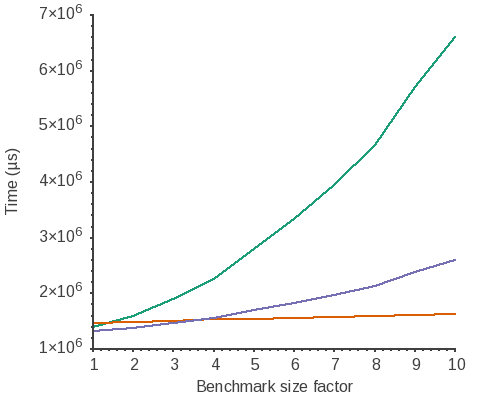
\includegraphics[scale=0.5]{images/bf-consecutive_loops.png}
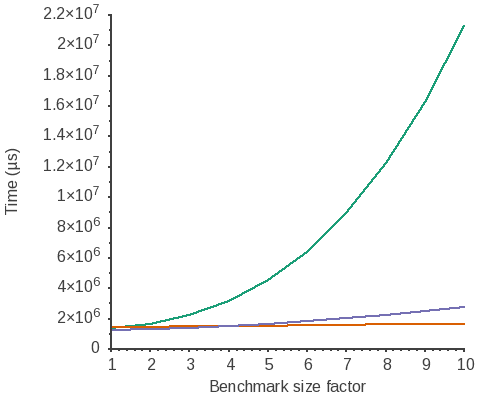
\includegraphics[scale=0.5]{images/bf-imbricated_loops.png}
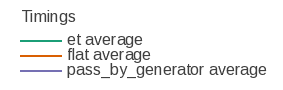
\includegraphics[scale=0.5]{images/bf-graph-legend.png}
\caption{
  Compiler execution time measurements for consecutive loops (left) and nested loops (right)
}\label{fig:bf-bench}
\end{figure}

Figure \ref{fig:bf-bench}
both highlight considerably higher compiler execution times for the expression
template based backend, high enough to suggest that the use of expression
templates induces an overhead higher than parsing and generating BF programs
using the pass-by-generator backend. However the pass-by-generator backend still
has a compile time overhead much higher than the flat backend, which shows near
constant compiler execution times on these small scale benchmarks.\\

Finally, AST deepening has a much higher impact on compile times than AST
widening with the expression template backends, whereas the other backends seem
to scale similarly as the AST grows wider or deeper.

\subsubsection{Realistic BF programs}

The following benchmarks consist in measuring compiler execution times for
compiling BF code examples. These example programs are also used to validate the
metacompiler's backend implementations by compiling them and verifying their
output.

\begin{itemize}
\item A Hello World program (106 tokens).
\item The same Hello World program, ran twice (212 tokens).
\item A Mandelbrot set fractal viewer (11672 tokens).
\end{itemize}

\begin{figure}[h]
\begin{tabular}{|c|c|c|c|}
\hline
Backend             & Hello World & Hello World x2  & Mandelbrot \\
\hline
Flat                & 1.81        & 2.25            & 49.68 \\
Pass-by-generator   & 9.77        & 34.37           & Failure (timeout) \\
Expression template & 50.60       & 192.73          & Failure (timeout) \\
\hline
\end{tabular}
\caption{BF compile time measurements in seconds
}\label{fig:BF-compile-times}
\end{figure}

The measurements in figure \ref{fig:BF-compile-times} help us better understand
how various metacompiling techniques behave at scale. The "Flat" backend shows
very good performance on all examples, including the Mandelbrot example that is
about 100 times larger than the Hello World example. However the other cases
highlight severe scaling issues and tend to confirm our previous hypothesis
being that using generator functions to pass values makes the code generation
quadratic. Finally, the "Expression template" backend performance highlights
heavy performance impact when expression templates are being used, which is
likely due to the complexity of the mechanisms expression templates involve like
SFINAE and overload resolution.

\subsection{Formula metacompiler evaluation}

The mathematical formula metacompiler uses a slighlty different code generation
technique. It can be used with or without Blaze, and Blaze can be used alone as
well. In this subsection we are therefore measuring compiler execution times for
the metacompiler for code generation using Blaze, but also for code generation
without Blaze by doing simple math operations on integers, and using Blaze
alone.

\subsubsection{Variable-size benchmark cases}

To evaluate the performance compile time impact of mathematical formula parsing,
we run benchmarks for two cases:

\begin{itemize}
\item \lstinline|no-formula-blaze|: Blaze code generation using the library's
      own API.
\item \lstinline|formula-blaze|: Blaze code generation from a formula parsed at
      compile time and transformed into a Blaze expression.
\end{itemize}

Both benchmarks consist in running a series of additions
\lstinline|x + y + ... x| with \lstinline|x + y + | repeated N times, and the
variables \lstinline|x| and \lstinline|y| of type
\lstinline|blaze::DynamicVector<unsigned int>|.

\begin{figure}[h]
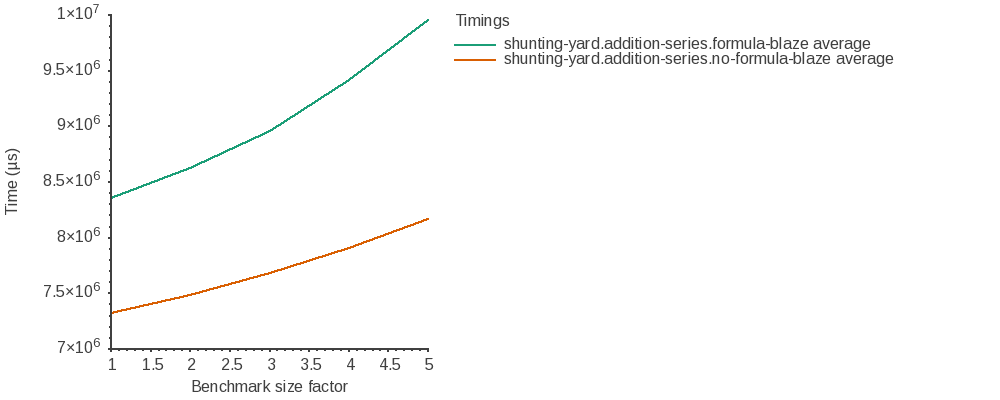
\includegraphics[scale=0.5]{
  images/shunting-yard.addition-series.graph.png
}
\caption{Execution time measurements for math formula compilation
}\label{fig:sy-rubbish-benchmark-graph}
\end{figure}

The figure \ref{fig:sy-rubbish-benchmark-graph} shows a compiler execution time
overhead of around 20\% when adding compile time parsing.
While it is noticeable, Blaze still accounts for most of the compiler execution
time.

\section{Conclusion}

We wanted to demonstrate that using \constexpr code to implement parsers for
\dsel of arbitrary syntax in \cpp23 is possible despite limitations on
\constexpr memory allocation, and that doing so is possible with reasonable
impact on compilation times.\\

We achieved that by implementing a \constexpr parser for the Brainfuck language,
with code generation backends implementing three different strategies to
transform \constexpr program representations into code using function
generators, expression templates, and non-type template parameters.
We also demonstrated the interoperability of these \constexpr parsers by
implementing a parser for mathematical languages that can be used as a frontend
for existing high performance \cpp computation libraries.\\

Our benchmarks highlight compilation time scaling issues with pass-by-generator
and expression template code generation strategies for large programs, and
excellent scaling capabilities for non-type template parameter based code
generation strategies. These results can be used to decide which strategy to
adopt for the implementation of future \dsel based on \constexpr parsers
based on considerations for compilation times or implementation complexity.\\

Going forward, \constexpr parser generators could help reduce
\dsel implementation time and help embed more languages into \cpp23.
Further research has to be made to determine the impact of such generators on
\dsel implementation complexity and compilation times.


%% Appendix
\appendix
\section{Appendix}

\subsection{BF parser implementation}\label{app:bf-parser}

\lstinputlisting[
  language=C++,
  firstline=26,
  lastline=62
]{external/poacher/brainfog/include/brainfog/parsers/naive.hpp}

\end{document}
